\documentclass[1p]{elsarticle_modified}
%\bibliographystyle{elsarticle-num}

%\usepackage[colorlinks]{hyperref}
%\usepackage{abbrmath_seonhwa} %\Abb, \Ascr, \Acal ,\Abf, \Afrak
\usepackage{amsfonts}
\usepackage{amssymb}
\usepackage{amsmath}
\usepackage{amsthm}
\usepackage{scalefnt}
\usepackage{amsbsy}
\usepackage{kotex}
\usepackage{caption}
\usepackage{subfig}
\usepackage{color}
\usepackage{graphicx}
\usepackage{xcolor} %% white, black, red, green, blue, cyan, magenta, yellow
\usepackage{float}
\usepackage{setspace}
\usepackage{hyperref}

\usepackage{tikz}
\usetikzlibrary{arrows}

\usepackage{multirow}
\usepackage{array} % fixed length table
\usepackage{hhline}

%%%%%%%%%%%%%%%%%%%%%
\makeatletter
\renewcommand*\env@matrix[1][\arraystretch]{%
	\edef\arraystretch{#1}%
	\hskip -\arraycolsep
	\let\@ifnextchar\new@ifnextchar
	\array{*\c@MaxMatrixCols c}}
\makeatother %https://tex.stackexchange.com/questions/14071/how-can-i-increase-the-line-spacing-in-a-matrix
%%%%%%%%%%%%%%%

\usepackage[normalem]{ulem}

\newcommand{\msout}[1]{\ifmmode\text{\sout{\ensuremath{#1}}}\else\sout{#1}\fi}
%SOURCE: \msout is \stkout macro in https://tex.stackexchange.com/questions/20609/strikeout-in-math-mode

\newcommand{\cancel}[1]{
	\ifmmode
	{\color{red}\msout{#1}}
	\else
	{\color{red}\sout{#1}}
	\fi
}

\newcommand{\add}[1]{
	{\color{blue}\uwave{#1}}
}

\newcommand{\replace}[2]{
	\ifmmode
	{\color{red}\msout{#1}}{\color{blue}\uwave{#2}}
	\else
	{\color{red}\sout{#1}}{\color{blue}\uwave{#2}}
	\fi
}

\newcommand{\Sol}{\mathcal{S}} %segment
\newcommand{\D}{D} %diagram
\newcommand{\A}{\mathcal{A}} %arc


%%%%%%%%%%%%%%%%%%%%%%%%%%%%%5 test

\def\sl{\operatorname{\textup{SL}}(2,\Cbb)}
\def\psl{\operatorname{\textup{PSL}}(2,\Cbb)}
\def\quan{\mkern 1mu \triangleright \mkern 1mu}

\theoremstyle{definition}
\newtheorem{thm}{Theorem}[section]
\newtheorem{prop}[thm]{Proposition}
\newtheorem{lem}[thm]{Lemma}
\newtheorem{ques}[thm]{Question}
\newtheorem{cor}[thm]{Corollary}
\newtheorem{defn}[thm]{Definition}
\newtheorem{exam}[thm]{Example}
\newtheorem{rmk}[thm]{Remark}
\newtheorem{alg}[thm]{Algorithm}

\newcommand{\I}{\sqrt{-1}}
\begin{document}

%\begin{frontmatter}
%
%\title{Boundary parabolic representations of knots up to 8 crossings}
%
%%% Group authors per affiliation:
%\author{Yunhi Cho} 
%\address{Department of Mathematics, University of Seoul, Seoul, Korea}
%\ead{yhcho@uos.ac.kr}
%
%
%\author{Seonhwa Kim} %\fnref{s_kim}}
%\address{Center for Geometry and Physics, Institute for Basic Science, Pohang, 37673, Korea}
%\ead{ryeona17@ibs.re.kr}
%
%\author{Hyuk Kim}
%\address{Department of Mathematical Sciences, Seoul National University, Seoul 08826, Korea}
%\ead{hyukkim@snu.ac.kr}
%
%\author{Seokbeom Yoon}
%\address{Department of Mathematical Sciences, Seoul National University, Seoul, 08826,  Korea}
%\ead{sbyoon15@snu.ac.kr}
%
%\begin{abstract}
%We find all boundary parabolic representation of knots up to 8 crossings.
%
%\end{abstract}
%\begin{keyword}
%    \MSC[2010] 57M25 
%\end{keyword}
%
%\end{frontmatter}

%\linenumbers
%\tableofcontents
%
\newcommand\colored[1]{\textcolor{white}{\rule[-0.35ex]{0.8em}{1.4ex}}\kern-0.8em\color{red} #1}%
%\newcommand\colored[1]{\textcolor{white}{ #1}\kern-2.17ex	\textcolor{white}{ #1}\kern-1.81ex	\textcolor{white}{ #1}\kern-2.15ex\color{red}#1	}

{\Large $\underline{11a_{265}~(K11a_{265})}$}

\setlength{\tabcolsep}{10pt}
\renewcommand{\arraystretch}{1.6}
\vspace{1cm}\begin{tabular}{m{100pt}>{\centering\arraybackslash}m{274pt}}
\multirow{5}{120pt}{
	\centering
	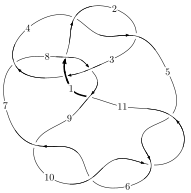
\includegraphics[width=112pt]{../../../GIT/diagram.site/Diagrams/png/514_11a_265.png}\\
\ \ \ A knot diagram\footnotemark}&
\allowdisplaybreaks
\textbf{Linearized knot diagam} \\
\cline{2-2}
 &
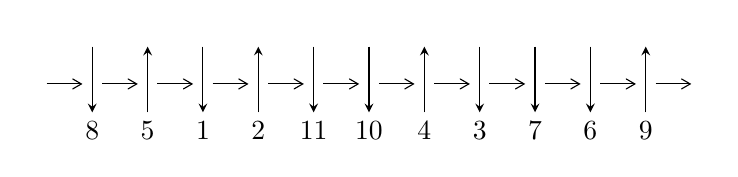
\begin{tikzpicture}[x=20pt, y=17pt]
	% nodes
	\node (C0) at (0, 0) {};
	\node (C1) at (1, 0) {};
	\node (C1U) at (1, +1) {};
	\node (C1D) at (1, -1) {8};

	\node (C2) at (2, 0) {};
	\node (C2U) at (2, +1) {};
	\node (C2D) at (2, -1) {5};

	\node (C3) at (3, 0) {};
	\node (C3U) at (3, +1) {};
	\node (C3D) at (3, -1) {1};

	\node (C4) at (4, 0) {};
	\node (C4U) at (4, +1) {};
	\node (C4D) at (4, -1) {2};

	\node (C5) at (5, 0) {};
	\node (C5U) at (5, +1) {};
	\node (C5D) at (5, -1) {11};

	\node (C6) at (6, 0) {};
	\node (C6U) at (6, +1) {};
	\node (C6D) at (6, -1) {10};

	\node (C7) at (7, 0) {};
	\node (C7U) at (7, +1) {};
	\node (C7D) at (7, -1) {4};

	\node (C8) at (8, 0) {};
	\node (C8U) at (8, +1) {};
	\node (C8D) at (8, -1) {3};

	\node (C9) at (9, 0) {};
	\node (C9U) at (9, +1) {};
	\node (C9D) at (9, -1) {7};

	\node (C10) at (10, 0) {};
	\node (C10U) at (10, +1) {};
	\node (C10D) at (10, -1) {6};

	\node (C11) at (11, 0) {};
	\node (C11U) at (11, +1) {};
	\node (C11D) at (11, -1) {9};
	\node (C12) at (12, 0) {};

	% arrows
	\draw[->,>={angle 60}]
	(C0) edge (C1) (C1) edge (C2) (C2) edge (C3) (C3) edge (C4) (C4) edge (C5) (C5) edge (C6) (C6) edge (C7) (C7) edge (C8) (C8) edge (C9) (C9) edge (C10) (C10) edge (C11) (C11) edge (C12) ;	\draw[->,>=stealth]
	(C1U) edge (C1D) (C2D) edge (C2U) (C3U) edge (C3D) (C4D) edge (C4U) (C5U) edge (C5D) (C6U) edge (C6D) (C7D) edge (C7U) (C8U) edge (C8D) (C9U) edge (C9D) (C10U) edge (C10D) (C11D) edge (C11U) ;
	\end{tikzpicture} \\
\hhline{~~} \\& 
\textbf{Solving Sequence} \\ \cline{2-2} 
 &
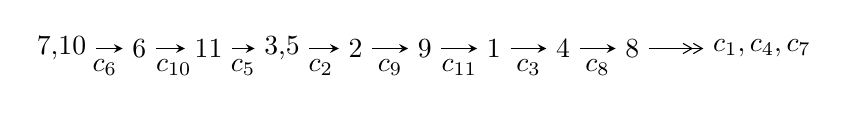
\begin{tikzpicture}[x=25pt, y=7pt]
	% node
	\node (A0) at (-1/8, 0) {7,10};
	\node (A1) at (1, 0) {6};
	\node (A2) at (2, 0) {11};
	\node (A3) at (49/16, 0) {3,5};
	\node (A4) at (33/8, 0) {2};
	\node (A5) at (41/8, 0) {9};
	\node (A6) at (49/8, 0) {1};
	\node (A7) at (57/8, 0) {4};
	\node (A8) at (65/8, 0) {8};
	\node (C1) at (1/2, -1) {$c_{6}$};
	\node (C2) at (3/2, -1) {$c_{10}$};
	\node (C3) at (5/2, -1) {$c_{5}$};
	\node (C4) at (29/8, -1) {$c_{2}$};
	\node (C5) at (37/8, -1) {$c_{9}$};
	\node (C6) at (45/8, -1) {$c_{11}$};
	\node (C7) at (53/8, -1) {$c_{3}$};
	\node (C8) at (61/8, -1) {$c_{8}$};
	\node (A9) at (10, 0) {$c_{1},c_{4},c_{7}$};

	% edge
	\draw[->,>=stealth]	
	(A0) edge (A1) (A1) edge (A2) (A2) edge (A3) (A3) edge (A4) (A4) edge (A5) (A5) edge (A6) (A6) edge (A7) (A7) edge (A8) ;
	\draw[->>,>={angle 60}]	
	(A8) edge (A9);
\end{tikzpicture} \\ 

\end{tabular} \\

\footnotetext{
The image of knot diagram is generated by the software ``\textbf{Draw programme}" developed by Andrew Bartholomew(\url{http://www.layer8.co.uk/maths/draw/index.htm\#Running-draw}), where we modified some parts for our purpose(\url{https://github.com/CATsTAILs/LinksPainter}).
}\phantom \\ \newline 
\centering \textbf{Ideals for irreducible components\footnotemark of $X_{\text{par}}$} 
 
\begin{align*}
I^u_{1}&=\langle 
-3051064229120 u^{53}-209833800856320 u^{52}+\cdots+578826226766096229 b+3885666844,\\
\phantom{I^u_{1}}&\phantom{= \langle  }-3.04606\times10^{12} u^{53}-2.09713\times10^{14} u^{52}+\cdots+5.78826\times10^{17} a+1.06118\times10^{18},\;u^{54}+u^{53}+\cdots+3 u+1\rangle \\
\\
\end{align*}
\raggedright * 1 irreducible components of $\dim_{\mathbb{C}}=0$, with total 54 representations.\\
\footnotetext{All coefficients of polynomials are rational numbers. But the coefficients are sometimes approximated in decimal forms when there is not enough margin.}
\newpage
\renewcommand{\arraystretch}{1}
\centering \section*{I. $I^u_{1}= \langle -3.05\times10^{12} u^{53}-2.10\times10^{14} u^{52}+\cdots+5.79\times10^{17} b+3.89\times10^{9},\;-3.05\times10^{12} u^{53}-2.10\times10^{14} u^{52}+\cdots+5.79\times10^{17} a+1.06\times10^{18},\;u^{54}+u^{53}+\cdots+3 u+1 \rangle$}
\flushleft \textbf{(i) Arc colorings}\\
\begin{tabular}{m{7pt} m{180pt} m{7pt} m{180pt} }
\flushright $a_{7}=$&$\begin{pmatrix}1\\0\end{pmatrix}$ \\
\flushright $a_{10}=$&$\begin{pmatrix}0\\u\end{pmatrix}$ \\
\flushright $a_{6}=$&$\begin{pmatrix}1\\- u^2\end{pmatrix}$ \\
\flushright $a_{11}=$&$\begin{pmatrix}- u\\u^3+u\end{pmatrix}$ \\
\flushright $a_{3}=$&$\begin{pmatrix}5.26248\times10^{-6} u^{53}+0.000362307 u^{52}+\cdots-2.47819 u-1.83333\\5.27112\times10^{-6} u^{53}+0.000362516 u^{52}+\cdots+3.16667 u-6.71301\times10^{-9}\end{pmatrix}$ \\
\flushright $a_{5}=$&$\begin{pmatrix}u^2+1\\- u^4-2 u^2\end{pmatrix}$ \\
\flushright $a_{2}=$&$\begin{pmatrix}1.21040\times10^{-6} u^{53}+0.0000804923 u^{52}+\cdots-3.23347 u-1.01667\\1.19100\times10^{-6} u^{53}+0.0000798962 u^{52}+\cdots+3.18333 u-1.72656\times10^{-9}\end{pmatrix}$ \\
\flushright $a_{9}=$&$\begin{pmatrix}u\\u\end{pmatrix}$ \\
\flushright $a_{1}=$&$\begin{pmatrix}u^5+2 u^3- u\\u^5+3 u^3+u\end{pmatrix}$ \\
\flushright $a_{4}=$&$\begin{pmatrix}-7.89546\times10^{-7} u^{53}-0.0000401538 u^{52}+\cdots-2.31083 u-1.75000\\-6.83885\times10^{-7} u^{53}-0.0000369648 u^{52}+\cdots+3.25000 u+1.91977\times10^{-9}\end{pmatrix}$ \\
\flushright $a_{8}=$&$\begin{pmatrix}-0.00581270 u^{53}-0.00326390 u^{52}+\cdots-0.253465 u+0.116715\\0.0000208391 u^{53}+0.00252101 u^{52}+\cdots+2.48502 u+0.00250009\end{pmatrix}$\\ \flushright $a_{8}=$&$\begin{pmatrix}-0.00581270 u^{53}-0.00326390 u^{52}+\cdots-0.253465 u+0.116715\\0.0000208391 u^{53}+0.00252101 u^{52}+\cdots+2.48502 u+0.00250009\end{pmatrix}$\\&\end{tabular}
\flushleft \textbf{(ii) Obstruction class $= -1$}\\~\\
\flushleft \textbf{(iii) Cusp Shapes $= -\frac{613554862282394952}{192942075588698743} u^{53}-\frac{459136890023638500}{192942075588698743} u^{52}+\cdots+\frac{755304846551017564}{192942075588698743} u+\frac{883739019103167146}{192942075588698743}$}\\~\\
\newpage\renewcommand{\arraystretch}{1}
\flushleft \textbf{(iv) u-Polynomials at the component}\newline \\
\begin{tabular}{m{50pt}|m{274pt}}
Crossings & \hspace{64pt}u-Polynomials at each crossing \\
\hline $$\begin{aligned}c_{1}\end{aligned}$$&$\begin{aligned}
&u^{54}+3 u^{53}+\cdots+u+1
\end{aligned}$\\
\hline $$\begin{aligned}c_{2},c_{4}\end{aligned}$$&$\begin{aligned}
&u^{54}+u^{53}+\cdots+9 u+1
\end{aligned}$\\
\hline $$\begin{aligned}c_{3}\end{aligned}$$&$\begin{aligned}
&u^{54}-9 u^{53}+\cdots- u+1
\end{aligned}$\\
\hline $$\begin{aligned}c_{5},c_{6},c_{9}\\c_{10}\end{aligned}$$&$\begin{aligned}
&u^{54}- u^{53}+\cdots-3 u+1
\end{aligned}$\\
\hline $$\begin{aligned}c_{7}\end{aligned}$$&$\begin{aligned}
&u^{54}-3 u^{53}+\cdots+15 u-1
\end{aligned}$\\
\hline $$\begin{aligned}c_{8}\end{aligned}$$&$\begin{aligned}
&u^{54}- u^{53}+\cdots-39 u+7
\end{aligned}$\\
\hline $$\begin{aligned}c_{11}\end{aligned}$$&$\begin{aligned}
&u^{54}+13 u^{53}+\cdots+657 u+99
\end{aligned}$\\
\hline
\end{tabular}\\~\\
\newpage\renewcommand{\arraystretch}{1}
\flushleft \textbf{(v) Riley Polynomials at the component}\newline \\
\begin{tabular}{m{50pt}|m{274pt}}
Crossings & \hspace{64pt}Riley Polynomials at each crossing \\
\hline $$\begin{aligned}c_{1}\end{aligned}$$&$\begin{aligned}
&y^{54}+9 y^{53}+\cdots+3 y+1
\end{aligned}$\\
\hline $$\begin{aligned}c_{2},c_{4}\end{aligned}$$&$\begin{aligned}
&y^{54}-35 y^{53}+\cdots-9 y+1
\end{aligned}$\\
\hline $$\begin{aligned}c_{3}\end{aligned}$$&$\begin{aligned}
&y^{54}-3 y^{53}+\cdots-9 y+1
\end{aligned}$\\
\hline $$\begin{aligned}c_{5},c_{6},c_{9}\\c_{10}\end{aligned}$$&$\begin{aligned}
&y^{54}+61 y^{53}+\cdots+3 y+1
\end{aligned}$\\
\hline $$\begin{aligned}c_{7}\end{aligned}$$&$\begin{aligned}
&y^{54}-55 y^{53}+\cdots-413 y+1
\end{aligned}$\\
\hline $$\begin{aligned}c_{8}\end{aligned}$$&$\begin{aligned}
&y^{54}-43 y^{53}+\cdots-317 y+49
\end{aligned}$\\
\hline $$\begin{aligned}c_{11}\end{aligned}$$&$\begin{aligned}
&y^{54}+5 y^{53}+\cdots+103347 y+9801
\end{aligned}$\\
\hline
\end{tabular}\\~\\
\newpage\flushleft \textbf{(vi) Complex Volumes and Cusp Shapes}
$$\begin{array}{c|c|c}  
\text{Solutions to }I^u_{1}& \I (\text{vol} + \sqrt{-1}CS) & \text{Cusp shape}\\
 \hline 
\begin{aligned}
u &= \phantom{-}0.545362 + 0.766936 I \\
a &= -0.188047 - 0.903445 I \\
b &= -0.949767 - 0.409626 I\end{aligned}
 & \phantom{-}1.00016 - 3.95703 I & -3.00000 + 11.79776 I \\ \hline\begin{aligned}
u &= \phantom{-}0.545362 - 0.766936 I \\
a &= -0.188047 + 0.903445 I \\
b &= -0.949767 + 0.409626 I\end{aligned}
 & \phantom{-}1.00016 + 3.95703 I & -3.00000 - 11.79776 I \\ \hline\begin{aligned}
u &= -0.172970 + 1.046260 I \\
a &= -1.181840 + 0.461864 I \\
b &= -0.428067 - 0.337725 I\end{aligned}
 & \phantom{-}5.26922 - 5.01222 I & \phantom{-0.000000 } 0 \\ \hline\begin{aligned}
u &= -0.172970 - 1.046260 I \\
a &= -1.181840 - 0.461864 I \\
b &= -0.428067 + 0.337725 I\end{aligned}
 & \phantom{-}5.26922 + 5.01222 I & \phantom{-0.000000 } 0 \\ \hline\begin{aligned}
u &= -0.561965 + 0.693690 I \\
a &= \phantom{-}0.31746 + 1.44112 I \\
b &= -1.53183 + 1.30909 I\end{aligned}
 & \phantom{-}2.46124 + 12.12320 I & \phantom{-}0.08589 - 9.41589 I \\ \hline\begin{aligned}
u &= -0.561965 - 0.693690 I \\
a &= \phantom{-}0.31746 - 1.44112 I \\
b &= -1.53183 - 1.30909 I\end{aligned}
 & \phantom{-}2.46124 - 12.12320 I & \phantom{-}0.08589 + 9.41589 I \\ \hline\begin{aligned}
u &= -0.506554 + 0.624526 I \\
a &= \phantom{-}0.086447 - 0.728121 I \\
b &= \phantom{-}1.52442 - 0.61745 I\end{aligned}
 & -1.47018 + 6.23173 I & -3.03340 - 8.93677 I \\ \hline\begin{aligned}
u &= -0.506554 - 0.624526 I \\
a &= \phantom{-}0.086447 + 0.728121 I \\
b &= \phantom{-}1.52442 + 0.61745 I\end{aligned}
 & -1.47018 - 6.23173 I & -3.03340 + 8.93677 I \\ \hline\begin{aligned}
u &= \phantom{-}0.670771 + 0.429255 I \\
a &= \phantom{-}0.279527 - 0.397115 I \\
b &= -0.026389 - 0.348007 I\end{aligned}
 & -0.67521 - 2.21346 I & -9.82154 + 8.24478 I \\ \hline\begin{aligned}
u &= \phantom{-}0.670771 - 0.429255 I \\
a &= \phantom{-}0.279527 + 0.397115 I \\
b &= -0.026389 + 0.348007 I\end{aligned}
 & -0.67521 + 2.21346 I & -9.82154 - 8.24478 I\\
 \hline 
 \end{array}$$\newpage$$\begin{array}{c|c|c}  
\text{Solutions to }I^u_{1}& \I (\text{vol} + \sqrt{-1}CS) & \text{Cusp shape}\\
 \hline 
\begin{aligned}
u &= -0.411382 + 0.638832 I \\
a &= \phantom{-}0.14437 - 1.44846 I \\
b &= \phantom{-}0.95232 - 1.40932 I\end{aligned}
 & \phantom{-}3.27194 + 4.12688 I & \phantom{-}4.58912 - 9.06876 I \\ \hline\begin{aligned}
u &= -0.411382 - 0.638832 I \\
a &= \phantom{-}0.14437 + 1.44846 I \\
b &= \phantom{-}0.95232 + 1.40932 I\end{aligned}
 & \phantom{-}3.27194 - 4.12688 I & \phantom{-}4.58912 + 9.06876 I \\ \hline\begin{aligned}
u &= \phantom{-}0.499596 + 0.521821 I \\
a &= -0.436226 - 0.083526 I \\
b &= \phantom{-}0.207048 + 0.493590 I\end{aligned}
 & -0.70487 - 1.75962 I & -4.58587 + 3.17454 I \\ \hline\begin{aligned}
u &= \phantom{-}0.499596 - 0.521821 I \\
a &= -0.436226 + 0.083526 I \\
b &= \phantom{-}0.207048 - 0.493590 I\end{aligned}
 & -0.70487 + 1.75962 I & -4.58587 - 3.17454 I \\ \hline\begin{aligned}
u &= -0.293339 + 0.635944 I \\
a &= \phantom{-}0.850317 - 1.011600 I \\
b &= -0.428431 - 0.192704 I\end{aligned}
 & \phantom{-}4.01735 + 0.63222 I & \phantom{-}7.39930 - 2.66782 I \\ \hline\begin{aligned}
u &= -0.293339 - 0.635944 I \\
a &= \phantom{-}0.850317 + 1.011600 I \\
b &= -0.428431 + 0.192704 I\end{aligned}
 & \phantom{-}4.01735 - 0.63222 I & \phantom{-}7.39930 + 2.66782 I \\ \hline\begin{aligned}
u &= -0.659334 + 0.232085 I \\
a &= \phantom{-}0.346734 - 1.144240 I \\
b &= \phantom{-}1.24395 + 0.77928 I\end{aligned}
 & \phantom{-}1.09662 - 8.00461 I & -2.60038 + 4.65248 I \\ \hline\begin{aligned}
u &= -0.659334 - 0.232085 I \\
a &= \phantom{-}0.346734 + 1.144240 I \\
b &= \phantom{-}1.24395 - 0.77928 I\end{aligned}
 & \phantom{-}1.09662 + 8.00461 I & -2.60038 - 4.65248 I \\ \hline\begin{aligned}
u &= \phantom{-}0.393123 + 0.559225 I \\
a &= \phantom{-}0.37563 + 4.16236 I \\
b &= \phantom{-}2.99641 + 0.60734 I\end{aligned}
 & \phantom{-}1.56763 - 1.75278 I & -6.2825 - 17.5292 I \\ \hline\begin{aligned}
u &= \phantom{-}0.393123 - 0.559225 I \\
a &= \phantom{-}0.37563 - 4.16236 I \\
b &= \phantom{-}2.99641 - 0.60734 I\end{aligned}
 & \phantom{-}1.56763 + 1.75278 I & -6.2825 + 17.5292 I\\
 \hline 
 \end{array}$$\newpage$$\begin{array}{c|c|c}  
\text{Solutions to }I^u_{1}& \I (\text{vol} + \sqrt{-1}CS) & \text{Cusp shape}\\
 \hline 
\begin{aligned}
u &= \phantom{-}0.148291 + 1.360240 I \\
a &= -0.709327 + 0.835990 I \\
b &= -0.329247 + 0.393163 I\end{aligned}
 & \phantom{-}4.94656 - 5.25128 I & \phantom{-0.000000 } 0 \\ \hline\begin{aligned}
u &= \phantom{-}0.148291 - 1.360240 I \\
a &= -0.709327 - 0.835990 I \\
b &= -0.329247 - 0.393163 I\end{aligned}
 & \phantom{-}4.94656 + 5.25128 I & \phantom{-0.000000 } 0 \\ \hline\begin{aligned}
u &= -0.000111 + 0.622884 I \\
a &= -0.308967 - 0.550291 I \\
b &= -0.810890 + 0.336840 I\end{aligned}
 & \phantom{-}1.31595 - 1.53064 I & \phantom{-}2.46645 + 4.42217 I \\ \hline\begin{aligned}
u &= -0.000111 - 0.622884 I \\
a &= -0.308967 + 0.550291 I \\
b &= -0.810890 - 0.336840 I\end{aligned}
 & \phantom{-}1.31595 + 1.53064 I & \phantom{-}2.46645 - 4.42217 I \\ \hline\begin{aligned}
u &= -0.541870 + 0.294917 I \\
a &= -0.16659 + 1.62943 I \\
b &= -0.870080 - 0.000654 I\end{aligned}
 & -2.42907 - 2.60276 I & -6.59954 + 2.27110 I \\ \hline\begin{aligned}
u &= -0.541870 - 0.294917 I \\
a &= -0.16659 - 1.62943 I \\
b &= -0.870080 + 0.000654 I\end{aligned}
 & -2.42907 + 2.60276 I & -6.59954 - 2.27110 I \\ \hline\begin{aligned}
u &= \phantom{-}0.615568\phantom{ +0.000000I} \\
a &= -0.465542\phantom{ +0.000000I} \\
b &= \phantom{-}0.796207\phantom{ +0.000000I}\end{aligned}
 & -1.10777\phantom{ +0.000000I} & -11.9580\phantom{ +0.000000I} \\ \hline\begin{aligned}
u &= -0.04794 + 1.44591 I \\
a &= \phantom{-}0.30412 - 1.67700 I \\
b &= \phantom{-}0.023300 - 0.933728 I\end{aligned}
 & \phantom{-}2.95011 - 0.80061 I & \phantom{-0.000000 } 0 \\ \hline\begin{aligned}
u &= -0.04794 - 1.44591 I \\
a &= \phantom{-}0.30412 + 1.67700 I \\
b &= \phantom{-}0.023300 + 0.933728 I\end{aligned}
 & \phantom{-}2.95011 + 0.80061 I & \phantom{-0.000000 } 0 \\ \hline\begin{aligned}
u &= \phantom{-}0.346728 + 0.415892 I \\
a &= -0.41230 - 2.49448 I \\
b &= -2.30227 + 0.40921 I\end{aligned}
 & \phantom{-}1.12331 - 0.98698 I & \phantom{-}7.38443 + 9.46034 I\\
 \hline 
 \end{array}$$\newpage$$\begin{array}{c|c|c}  
\text{Solutions to }I^u_{1}& \I (\text{vol} + \sqrt{-1}CS) & \text{Cusp shape}\\
 \hline 
\begin{aligned}
u &= \phantom{-}0.346728 - 0.415892 I \\
a &= -0.41230 + 2.49448 I \\
b &= -2.30227 - 0.40921 I\end{aligned}
 & \phantom{-}1.12331 + 0.98698 I & \phantom{-}7.38443 - 9.46034 I \\ \hline\begin{aligned}
u &= \phantom{-}0.496604\phantom{ +0.000000I} \\
a &= -0.826100\phantom{ +0.000000I} \\
b &= \phantom{-}0.696774\phantom{ +0.000000I}\end{aligned}
 & -1.13235\phantom{ +0.000000I} & -10.5020\phantom{ +0.000000I} \\ \hline\begin{aligned}
u &= \phantom{-}0.07837 + 1.54926 I \\
a &= \phantom{-}1.86936 + 1.70184 I \\
b &= \phantom{-}2.37253 + 0.73488 I\end{aligned}
 & \phantom{-}7.92145 - 2.31500 I & \phantom{-0.000000 } 0 \\ \hline\begin{aligned}
u &= \phantom{-}0.07837 - 1.54926 I \\
a &= \phantom{-}1.86936 - 1.70184 I \\
b &= \phantom{-}2.37253 - 0.73488 I\end{aligned}
 & \phantom{-}7.92145 + 2.31500 I & \phantom{-0.000000 } 0 \\ \hline\begin{aligned}
u &= \phantom{-}0.13720 + 1.55270 I \\
a &= \phantom{-}0.040303 - 0.953011 I \\
b &= -0.542375 - 0.985698 I\end{aligned}
 & \phantom{-}6.29079 - 4.01270 I & \phantom{-0.000000 } 0 \\ \hline\begin{aligned}
u &= \phantom{-}0.13720 - 1.55270 I \\
a &= \phantom{-}0.040303 + 0.953011 I \\
b &= -0.542375 + 0.985698 I\end{aligned}
 & \phantom{-}6.29079 + 4.01270 I & \phantom{-0.000000 } 0 \\ \hline\begin{aligned}
u &= -0.04879 + 1.56688 I \\
a &= \phantom{-}1.45840 - 1.17346 I \\
b &= \phantom{-}1.72999 - 1.25663 I\end{aligned}
 & \phantom{-}8.64965 - 1.05444 I & \phantom{-0.000000 } 0 \\ \hline\begin{aligned}
u &= -0.04879 - 1.56688 I \\
a &= \phantom{-}1.45840 + 1.17346 I \\
b &= \phantom{-}1.72999 + 1.25663 I\end{aligned}
 & \phantom{-}8.64965 + 1.05444 I & \phantom{-0.000000 } 0 \\ \hline\begin{aligned}
u &= \phantom{-}0.10731 + 1.56661 I \\
a &= -2.89723 - 2.74617 I \\
b &= -2.89407 - 0.64960 I\end{aligned}
 & \phantom{-}8.80102 - 3.53795 I & \phantom{-0.000000 } 0 \\ \hline\begin{aligned}
u &= \phantom{-}0.10731 - 1.56661 I \\
a &= -2.89723 + 2.74617 I \\
b &= -2.89407 + 0.64960 I\end{aligned}
 & \phantom{-}8.80102 + 3.53795 I & \phantom{-0.000000 } 0\\
 \hline 
 \end{array}$$\newpage$$\begin{array}{c|c|c}  
\text{Solutions to }I^u_{1}& \I (\text{vol} + \sqrt{-1}CS) & \text{Cusp shape}\\
 \hline 
\begin{aligned}
u &= -0.14576 + 1.57745 I \\
a &= -1.40684 + 1.66633 I \\
b &= -2.06161 + 1.25521 I\end{aligned}
 & \phantom{-}5.94961 + 8.61448 I & \phantom{-0.000000 } 0 \\ \hline\begin{aligned}
u &= -0.14576 - 1.57745 I \\
a &= -1.40684 - 1.66633 I \\
b &= -2.06161 - 1.25521 I\end{aligned}
 & \phantom{-}5.94961 - 8.61448 I & \phantom{-0.000000 } 0 \\ \hline\begin{aligned}
u &= -0.08890 + 1.58461 I \\
a &= \phantom{-}0.610813 + 0.478237 I \\
b &= \phantom{-}1.332270 + 0.248255 I\end{aligned}
 & \phantom{-}11.59780 + 2.07370 I & \phantom{-0.000000 } 0 \\ \hline\begin{aligned}
u &= -0.08890 - 1.58461 I \\
a &= \phantom{-}0.610813 - 0.478237 I \\
b &= \phantom{-}1.332270 - 0.248255 I\end{aligned}
 & \phantom{-}11.59780 - 2.07370 I & \phantom{-0.000000 } 0 \\ \hline\begin{aligned}
u &= -0.11679 + 1.58495 I \\
a &= -0.47013 + 2.67136 I \\
b &= -0.82660 + 2.34169 I\end{aligned}
 & \phantom{-}10.82650 + 6.06392 I & \phantom{-0.000000 } 0 \\ \hline\begin{aligned}
u &= -0.11679 - 1.58495 I \\
a &= -0.47013 - 2.67136 I \\
b &= -0.82660 - 2.34169 I\end{aligned}
 & \phantom{-}10.82650 - 6.06392 I & \phantom{-0.000000 } 0 \\ \hline\begin{aligned}
u &= -0.372639 + 0.159058 I \\
a &= -1.55778 + 0.98703 I \\
b &= -0.893238 - 0.244729 I\end{aligned}
 & \phantom{-}2.00449 - 1.26243 I & -0.21146 + 2.28876 I \\ \hline\begin{aligned}
u &= -0.372639 - 0.159058 I \\
a &= -1.55778 - 0.98703 I \\
b &= -0.893238 + 0.244729 I\end{aligned}
 & \phantom{-}2.00449 + 1.26243 I & -0.21146 - 2.28876 I \\ \hline\begin{aligned}
u &= -0.16943 + 1.60101 I \\
a &= \phantom{-}0.78343 - 2.47982 I \\
b &= \phantom{-}1.68631 - 1.83629 I\end{aligned}
 & \phantom{-}10.1949 + 14.8555 I & \phantom{-0.000000 } 0 \\ \hline\begin{aligned}
u &= -0.16943 - 1.60101 I \\
a &= \phantom{-}0.78343 + 2.47982 I \\
b &= \phantom{-}1.68631 + 1.83629 I\end{aligned}
 & \phantom{-}10.1949 - 14.8555 I & \phantom{-0.000000 } 0\\
 \hline 
 \end{array}$$\newpage$$\begin{array}{c|c|c}  
\text{Solutions to }I^u_{1}& \I (\text{vol} + \sqrt{-1}CS) & \text{Cusp shape}\\
 \hline 
\begin{aligned}
u &= \phantom{-}0.16913 + 1.62019 I \\
a &= \phantom{-}0.64236 + 1.39992 I \\
b &= \phantom{-}1.033010 + 0.913072 I\end{aligned}
 & \phantom{-}9.06286 - 6.69333 I & \phantom{-0.000000 } 0 \\ \hline\begin{aligned}
u &= \phantom{-}0.16913 - 1.62019 I \\
a &= \phantom{-}0.64236 - 1.39992 I \\
b &= \phantom{-}1.033010 - 0.913072 I\end{aligned}
 & \phantom{-}9.06286 + 6.69333 I & \phantom{-0.000000 } 0 \\ \hline\begin{aligned}
u &= -0.01419 + 1.65792 I \\
a &= \phantom{-}0.271821 + 0.270288 I \\
b &= -0.453188 + 0.515678 I\end{aligned}
 & \phantom{-}14.5155 - 4.5567 I & \phantom{-0.000000 } 0 \\ \hline\begin{aligned}
u &= -0.01419 - 1.65792 I \\
a &= \phantom{-}0.271821 - 0.270288 I \\
b &= -0.453188 - 0.515678 I\end{aligned}
 & \phantom{-}14.5155 + 4.5567 I & \phantom{-0.000000 } 0\\
 \hline 
 \end{array}$$\newpage
\newpage\renewcommand{\arraystretch}{1}
\centering \section*{ II. u-Polynomials}
\begin{tabular}{m{50pt}|m{274pt}}
Crossings & \hspace{64pt}u-Polynomials at each crossing \\
\hline $$\begin{aligned}c_{1}\end{aligned}$$&$\begin{aligned}
&u^{54}+3 u^{53}+\cdots+u+1
\end{aligned}$\\
\hline $$\begin{aligned}c_{2},c_{4}\end{aligned}$$&$\begin{aligned}
&u^{54}+u^{53}+\cdots+9 u+1
\end{aligned}$\\
\hline $$\begin{aligned}c_{3}\end{aligned}$$&$\begin{aligned}
&u^{54}-9 u^{53}+\cdots- u+1
\end{aligned}$\\
\hline $$\begin{aligned}c_{5},c_{6},c_{9}\\c_{10}\end{aligned}$$&$\begin{aligned}
&u^{54}- u^{53}+\cdots-3 u+1
\end{aligned}$\\
\hline $$\begin{aligned}c_{7}\end{aligned}$$&$\begin{aligned}
&u^{54}-3 u^{53}+\cdots+15 u-1
\end{aligned}$\\
\hline $$\begin{aligned}c_{8}\end{aligned}$$&$\begin{aligned}
&u^{54}- u^{53}+\cdots-39 u+7
\end{aligned}$\\
\hline $$\begin{aligned}c_{11}\end{aligned}$$&$\begin{aligned}
&u^{54}+13 u^{53}+\cdots+657 u+99
\end{aligned}$\\
\hline
\end{tabular}\newpage\renewcommand{\arraystretch}{1}
\centering \section*{ III. Riley Polynomials}
\begin{tabular}{m{50pt}|m{274pt}}
Crossings & \hspace{64pt}Riley Polynomials at each crossing \\
\hline $$\begin{aligned}c_{1}\end{aligned}$$&$\begin{aligned}
&y^{54}+9 y^{53}+\cdots+3 y+1
\end{aligned}$\\
\hline $$\begin{aligned}c_{2},c_{4}\end{aligned}$$&$\begin{aligned}
&y^{54}-35 y^{53}+\cdots-9 y+1
\end{aligned}$\\
\hline $$\begin{aligned}c_{3}\end{aligned}$$&$\begin{aligned}
&y^{54}-3 y^{53}+\cdots-9 y+1
\end{aligned}$\\
\hline $$\begin{aligned}c_{5},c_{6},c_{9}\\c_{10}\end{aligned}$$&$\begin{aligned}
&y^{54}+61 y^{53}+\cdots+3 y+1
\end{aligned}$\\
\hline $$\begin{aligned}c_{7}\end{aligned}$$&$\begin{aligned}
&y^{54}-55 y^{53}+\cdots-413 y+1
\end{aligned}$\\
\hline $$\begin{aligned}c_{8}\end{aligned}$$&$\begin{aligned}
&y^{54}-43 y^{53}+\cdots-317 y+49
\end{aligned}$\\
\hline $$\begin{aligned}c_{11}\end{aligned}$$&$\begin{aligned}
&y^{54}+5 y^{53}+\cdots+103347 y+9801
\end{aligned}$\\
\hline
\end{tabular}
\vskip 2pc
\end{document}